\doublespacing % Do not change - required

\chapter{Future work and Substainability and Environment impact}
\label{ch5}

%%%%%%%%%%%%%%%%%%%%%%%%%%%%%%%%%%%%%%%
% IMPORTANT
\begin{spacing}{1} %THESE FOUR
\minitoc % LINES MUST APPEAR IN
\end{spacing} % EVERY
\thesisspacing % CHAPTER
% COPY THEM IN ANY NEW CHAPTER
%%%%%%%%%%%%%%%%%%%%%%%%%%%%%%%%%%%%%%%


\section{Future Improvements}
In summary, the future work can be concluded in Figure \ref{fig:future-work-roadmap}

\begin{figure}[htbp]
    \centering
    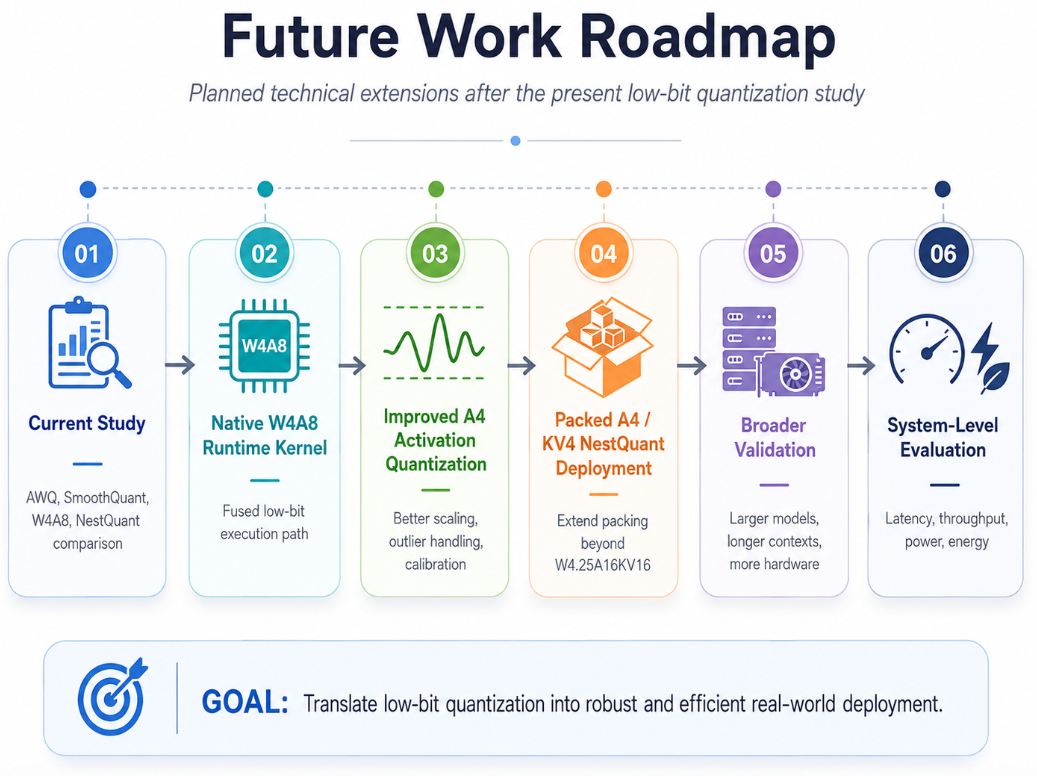
\includegraphics[width=0.95\textwidth]
    {imgs/future-work-roadmap.png}
    \caption{Future work roadmap.}
    \label{fig:future-work-roadmap}
\end{figure}

\subsection{Native Low-Bit Runtime Kernels}

The project-specific W4A8 pipeline currently combines packed INT4
weights with a separate dynamic INT8 activation-quantization stage.
Although this provides substantial memory compression, the execution
path is not a fully fused native INT4-by-INT8 matrix-multiplication
kernel.

A major future improvement is therefore the development of a fused W4A8
runtime kernel that directly consumes packed INT4 weights and INT8
activations. Such an implementation could reduce intermediate
quantize--dequantize operations, kernel-launch overhead and unnecessary
data movement. Similar optimisation could also be applied to the packed
NestQuant representation so that the low-bit format is exploited more
directly during inference.


\subsection{Improved Activation Quantization}

The NestQuant scope ablation showed that activation quantization was more
quality-sensitive than KV-cache quantization. Reducing activation
precision from A16 to A4 produced a substantially larger perplexity
increase than reducing the KV cache from KV16 to KV4.

Future development should therefore prioritise the A4 path. Possible
directions include improved activation scaling, more robust outlier
handling, layer-dependent quantization parameters and further
optimisation of the QA-LDLQ calibration procedure. The objective is to
reduce the additional quality penalty introduced by low-bit activations
while retaining the broader W/A/KV quantization scope.


\subsection{Extended Packed NestQuant Deployment}

The packed deployment experiments in this study focused on the
W4.25A16KV16 configuration. Future work should extend the packed
representation to the A4 and KV4 configurations so that
W4.25A16KV4, W4.25A4KV16 and W4.25A4KV4 can be evaluated using genuine
low-bit runtime implementations rather than quality-reference paths
alone.

This would allow the numerical benefits of broader NestQuant
quantization to be connected directly with physical memory, storage and
execution characteristics.


\subsection{Broader Experimental Validation}

The present experiments focus on Llama-3.2-3B-Instruct under a fixed
evaluation framework. Future work should evaluate the same methodology
across larger model sizes, alternative model families, longer context
lengths and different GPU architectures.

A broader evaluation should also include matched latency, throughput,
power and energy measurements. This would provide a more complete
assessment of whether reductions in numerical precision translate into
end-to-end deployment efficiency.


\section{Sustainability and Environmental Impact}
The sustainability relevance of low-bit quantization arises primarily
from its potential to reduce the computational resources required for
large-language-model deployment. Modern LLM inference is strongly
affected by model storage, GPU-memory capacity and data movement.
Reducing the physical representation of model tensors can therefore
improve hardware utilisation and potentially lower the resources
required to serve a given model.


\subsection{Computational Resource Efficiency}

The experimental results demonstrate substantial reductions in model
storage and GPU-memory requirements. Across the principal comparison,
the packed W4 configurations reduced runtime model-tensor storage by
approximately 64\% and peak GPU memory by approximately 61\% relative
to BF16.

The dedicated packed NestQuant implementation similarly reduced
checkpoint size from 5.78~GiB to 2.16~GiB and peak GPU memory from
6.01~GiB to 2.84~GiB.

These reductions can improve deployment efficiency by allowing a model
to operate within a smaller memory budget. In practical systems, this
may increase the range of hardware capable of hosting the model or allow
greater utilisation of an existing accelerator.


\subsection{Potential Environmental Benefits}

Lower storage and memory requirements may also reduce the amount of data
that must be transferred between memory and processing units during
inference. Since data movement is an important component of modern
accelerator workloads, effective low-bit representations have the
potential to reduce the computational resources associated with model
serving.

More memory-efficient models may additionally reduce the need for
high-capacity accelerator hardware for some deployment scenarios and
may extend the useful deployment range of existing hardware. These
effects could contribute indirectly to lower resource consumption when
low-bit quantization is deployed at scale.


\subsection{Environmental Limitations}

The present study did not directly measure electrical power, total
energy consumption or carbon emissions. The observed reductions in
checkpoint size and GPU-memory demand should therefore be interpreted as
evidence of improved computational-resource efficiency rather than as
direct measurements of environmental impact.

Quantization itself also introduces additional costs through calibration,
model conversion and implementation development. Furthermore, improved
inference efficiency can reduce the cost of model deployment and thereby
increase total model usage. This potential rebound effect means that a
reduction in resource consumption per inference does not necessarily
imply a proportional reduction in total system-level energy consumption.

Future sustainability assessment should therefore combine memory and
performance measurements with direct GPU power monitoring, energy per
token, workload utilisation and location-dependent carbon-intensity
estimates.